\chapter{Simulazione di un sistema complesso basato su Agenti}
\section{Introduzione}
Iniziamo analizzando un esempio di sistema complesso ovvero il movimento delle
folle di persone.

I sistemi complessi sono composti da tanti elementi che si integrano e collaborano.
Oltre a questo si ha la non linearità, una struttura gerarchica o connessa, si
ha robustezza e plasticità del sistema.
\subsection{Feedback}
Un sistema complesso ha la possibilità di osservare dei \textbf{feedback} che
possono essere positivi o negativi dal sistema.
\begin{esempio}
      Ipotizziamo di dover scegliere tra tre ristoranti e stiamo osservando
      le seguenti situazioni:
      \begin{itemize}
            \item Il primo ristorante è completamente vuoto.
            \item Il secondo ristorante è abbastanza affollato ma non è pieno.
            \item Il terzo ristorante è pieno e c'è una fila fuori.
      \end{itemize}
      In questo caso il feedback positivo è rappresentato dal secondo ristorante
      che è abbastanza affollato, quindi è probabile che sia buono. Il feedback
      negativo è rappresentato dal terzo e dal primo ristorante i quali
      rappresentano situazioni opposte ma entrambe possono essere viste come
      negative.
\end{esempio}
I feedback si possono ottenere come output del sistema, e in determinate circostanze,
può essere utile fornire in input tale valore per modificare l'ambiente o le
scelte che l'agente effettua. Ad esempio, un feedback positivo può amplificare
l'effetto di una scelta, mentre un feedback negativo può ridurre l'effetto di
una scelta. Quindi si hanno meccanismi di inibizione e stimolazione nel sistema.
\subsection{Motivazioni}
La ricerca e lo studio dei sistemi complessi è utile per chi si occupa di progettare,
pianificare e sviluppare , come ad esempio gli ingegneri, prodotti in quanto
permette di prendere spunto dai sistemi naturali per quelli artificiali.

L'obiettivo di questo studio è quello di studiare attraverso la simulazione del
modello quello che potrebbe essere il comportamento del sistema reale. Questo
permette di evitare di dover effettuare test sul sistema reale, che potrebbero
essere pericolosi o costosi.
\begin{esempio}
      Lo studio delle simulazioni del movimento delle folle di persone permette
      ad esempio di studiare il comportamento in caso di evacuazione di un edificio
      in caso di emergenza senza dover mettere in pericolo le persone.
\end{esempio}
\subsection{Folla di persone come sistema complesso}
La folla di persone è un sistema complesso perché è composto da tanti agenti,
ovvero i pedoni, che possono prendere decisioni individualmente o in gruppo. Oltre
a ciò, il comportamento delle persone può essere influenzato dall'ambiente in
cui si trovano. In generale, il comportamento delle folle è difficile da prevedere
perché è influenzato da molti fattori.

Quando si studia la folla si devono anche considerare situazioni di competizione
per lo spazio condiviso, ma anche di cooperazione per evitare situazioni di
stallo.

Inoltre, i pedoni possono avere stimoli di imitazione verso altri agenti, ad
esempio, se un pedone vede un altro attraversare la strada, potrebbe decidere
di attraversare anche lui. È anche possibile osservare una tendenza a stare a
distanza dagli altri.

Possiamo avere anche dei \textbf{fenomeni emergenti}, ovvero comportamenti che
si osservano a livello globale ma che non sono direttamente riconducibili al
comportamento degli agenti singoli. Ad esempio la ola degli stadi. Questo fenomeno
è risultante da un comportamento aggregato di tanti agenti, non si riconosce la
derivazione dal singolo.
\section{Simulazione}
\begin{definizione}[\textbf{Modello Computazionale}]
      Un \textbf{modello computazionale} è un qualcosa di sufficientemente ben
      definito per essere implementato.
\end{definizione}
\begin{definizione}[\textbf{Simulazione}]
      La \textbf{simulazione} al computer è un modo per sfruttare un modello
      computazionale, con lo scopo di:
      \begin{itemize}
            \item Valutare piani e design prima di effettivamente metterli in
                  pratica nel mondo reale.
            \item Valutare teorie e modelli esistenti di un sistema complesso
                  attraverso l'analisi degli effetti delle scelte modellistiche.
                  Un esempio è la ricerca della cura di una cellula attraverso
                  dei processi chimici, si potrebbe simulare l'ambiente per
                  capire come funziona.
      \end{itemize}
\end{definizione}
L'uso dell'ambiente simulato risulta a volte necessario perché il sistema reale
non può essere osservato, ad esempio quando lo si sta progettando o per motivi
etici o pratici.

Vogliamo ora analizzare il ciclo vita del processo di simulazione riportato in
figura \ref{fig:ciclo_simulazione}. Tale processo è composto dalle seguenti fasi:
\begin{itemize}
      \item Si parte da un sistema reale o da una sua porzione anche detta
            \textbf{Target System}.
      \item Partendo dal target system si costruisce un modello che rappresenta
            il sistema reale. Questo modello può essere di diversi tipi (es.
            fisico, matematico, algoritmico, ad agenti).
      \item Si implementa il modello, creando un simulatore.
      \item Una volta implementato il simulatore lo si esegue la simulazione,
            usando diverse condizioni iniziali. Per ogni esecuzione vengono
            generati dei dati di simulazione.
      \item Ottenuti i dati si analizzano e si confrontano con il target system.
            In questo modo valuto il simulatore utilizzando delle informazioni
            reali. Se i risultati ottenuti da questa analisi sono soddisfacenti
            allora posso usarlo per fini predittivi e di spiegazione.
\end{itemize}
\begin{figure}[!ht]
      \centering
      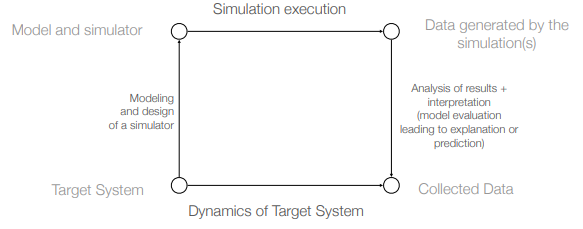
\includegraphics[width=0.5\textwidth]{./img/sim/ciclobase.png}
      \caption{Ciclo di vita della simulazione}
      \label{fig:ciclo_simulazione}
\end{figure}

Il processo di simulazione che abbiamo analizzato, lo possiamo suddividere nelle
seguenti macro-categorie:
\begin{itemize}
      \item \textbf{Sintesi}: si azzarda una sintesi del sistema reale e si crea
            un simulatore, formalizzo i fenomeni del sistema, ciò mi permette di
            definire indicatori, metriche.
      \item \textbf{Analisi}: si analizzano i risultati ottenuti dal simulatore e
            li confronto con i dati reali per validare i simulatori.
\end{itemize}
\begin{figure}[!ht]
      \centering
      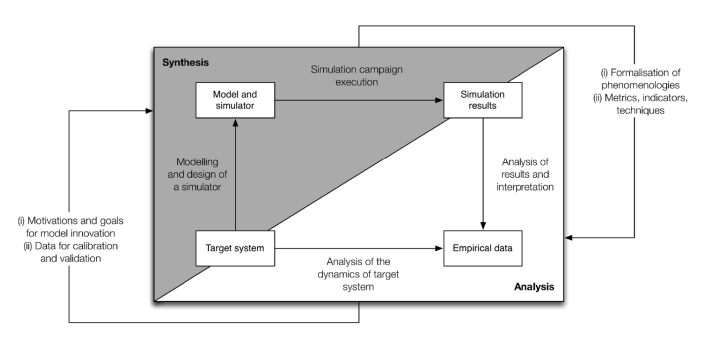
\includegraphics[width=0.7\textwidth]{./img/sim/lifecycle.png}
      \caption{Sintesi e Analisi}
      \label{fig:sintesi_analisi}
\end{figure}

Per quanto riguarda l'analisi delle folle possiamo definire i seguenti livelli:s
\begin{itemize}
      \item \textbf{Livello operazionale}: rappresenta l'insieme di azioni che
            sono definite nel sistema, come ad esempio camminare, aspettare,
            effettuare un'attività, scelta della traiettoria a livello geometrico
            e ad ostacoli. (agente semplice)
      \item \textbf{Livello tattico} (pianifico): si discretizza il livello
            precedente spesso in un grafo, aggiungendo uno scheduling delle
            attività, scelta della strada. È quindi richiesta una base di
            conoscenza.
      \item \textbf{Livello strategico}
\end{itemize}
\begin{figure}[!ht]
      \centering
      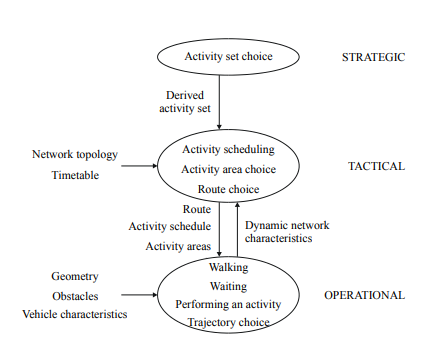
\includegraphics[width=0.5\textwidth]{./img/sim/levelsAnalysis.png}
      \caption{Livelli di analisi delle folle}
      \label{fig:livelli_folle}
\end{figure}

Le folle di persone possono essere modellate sotto diversi aspetti, ad esempio:
\begin{itemize}
      \item \textbf{Macroscopico}: modello solamente gli aspetti globali della
            folla, spesso si specificano dei vincoli a livello globale, attraverso
            un sistema di equazioni differenziali. Ha diversi problemi:
            \begin{itemize}
                  \item Gli agenti hanno lo stesso obiettivo e comportamento.
                  \item Risulta difficile considerare gli aspetti dinamici
                        dell'ambiente perché dovremo specificare un nuovo sistema
                        differenziale che modella il secondo stato dell'ambiente
                        e abilitare i singoli sistemi in base alla tempo.
                  \item Non si riescono a considerare tutti gli aspetti dinamici
                        della folla.
                  \item Utile per risolvere problemi di ottimizzazione nei contesti
                        specifici.
            \end{itemize}
            Spesso sono simulazioni approssimative, si fa variare il tempo e si
            prende uno screenshot del modello a due tempi differenti. Buone
            prestazioni computazionali perché sono indipendenti dal numero
            di pedoni, però sono più limitati.
      \item \textbf{Microscopico}: si specifica il modello dei singoli agenti
            secondo la loro architettura e devo tenere traccia degli agenti.
            Serve maggior attenzione sul sistema modellato per renderlo
            compatibile con la versione macroscopica.

            Con questo modello si possono sempre generare le stesse dinamiche
            aggregate della modellazione macroscopica. La modellazione
            microscopica può essere realizzata in diversi modi:
            \begin{itemize}
                  \item \textbf{Particelle}: gli agenti sono rappresentati da
                        particelle. Questa soluzione permette di mantenere la
                        componente fisica, ma si modellano i singoli e non le
                        componenti aggregate. Si specifica una velocità delle
                        particelle e si applicano delle forse su di esse anche in
                        base ai vicini. Le forze sono generate dagli obiettivi e dalle
                        altre particelle.
                  \item \textbf{Automi cellulari}
            \end{itemize}
      \item \textbf{Mesoscopiche}: rappresenta una via di mezzo tra le precedenti
            due. Si modellano i singoli agenti ma si considerano anche le componenti
            aggregate. Si considerano le interazioni tra gli agenti e le componenti
            globali. Si ha però un dettaglio inferiore sulla rappresentazione
            spaziale.
\end{itemize}
Per complicare i simulatori, perché ho parametri liberi, non posso modellare
l'eterogeneità, non posso specificare strutture particolari dell'ambiente \dots
\begin{nota}
      Non esiste un approccio modellistico migliore, dipende tutto da quanto
      conosciamo il fenomeno, gli obiettivi e i dati che abbiamo o misuriamo.
\end{nota}
Il processo di definizione dei simulatori coinvolge diverse fasi, regole e
tipologie di conoscenze. I passaggi tra i diversi livelli di astrazione possono
portare all'introduzione di errori e di incertezze.

\section{Reinforcement learning per la gestione temporizzata dei semafori}
L'ambiente è stato realizzato con SUMO, si ha un solo agente che guarda l'ambiente 
SUMO (al suo interno tanti agenti) e un decisore che invia all'agente le informazioni 
sulla temporizzazione corretta. Una semplificazione del simulatore è che non ci sono 
pedoni e non si guarda oltre l'incrocio.

Il tutto si basa sul cambiare stato ogni 10s e quando cambia deve mettere 4s di 
giallo.

Di algoritmi per RL ne esistono molti Q-Learning associo ad ogni azione 
una funzione di valore, maggiore è il valore allora migliore.

$\phi \in [0,1]$ se $\phi=0$ allora considero solo la nuova azione, $\phi=1$ 
allora la prima azione conta quanto l'ultima. Dal momento che la definizione dipende 
dalle azioni future, se lo spazio è ridotto allora si esplora tutta la combinatoria 
altrimenti si usa una rete neurale che mi approssima tutto.

Il problema è che gli stati dell'ambiente sono molto correlati rispetto al tempo 
quindi la rete ha un bias. Per il problema salviamo ogni sample (stato, azione, 
reward, stato prossimo) in un buffer e poi si allena la rete estraendo casualmente 
il sample.

\section{Reinforcement learning per la simulazione di pedoni}
Ho un modello regressivo che mi gestisce il cammino. 

PEr muoversi nell'ambiente ciascun agente ha la posizione del goal, dei vicini con 
le loro direzioni e dell'ostacolo più vicino. L'agente ha un raggio di visione e un 
cambiamento discreto della velocità.

L'apprendimento per rinforzo si articola attraverso le osservazioni che possono 
specificare gli stati dell'ambiente, l'agente ha una policy (funzione che massimizza 
la reward cumulata) e il reinforcement learning modifica la policy.

La tipologia di osservazioni sono:
\begin{itemize}
      \item intrinsica (velocità di movimento dell'agente)
      \item obiettivi e muri: distanza e codifica del tipo di oggetto (influenza la scelta dell'angolo)
      \item agenti e muri: distanza, tipo, direzione e velocità
\end{itemize}

L'agente regola la propria velocità di camminata in maniera continua e quindi
modifica il vettore e l'angolo.

La funzione obiettivo deve spesso essere: obiettivo molto alto positivo e tutto 
il resto un valore negativo. Si cerca di dare i valori negativi piuttosto che 
valori positivi per evitare massimi locali.

L'apprendimento per scenari differenti con CV e si nota che ogni volta che si cambia 
scenario otteniamo dei peggioramenti su reward ma permette di generalizzare bene 
e ridurre i tempi di apprendimento.

\section{Modellazione di sistemi eterogenei}
modellare l'attraversamento pedonale che è un sistema composto da due diverse tipologie 
di agente: macchina e pedone. Possono essere visti come due modelli distinti con 
delle conflict zone in cui i modelli si parlano.

I veicoli possono essere modellati come automi cellulari.

I pedoni possono essere modellati sempre con automi cellulari.

Bisogna specificare delle regole di interazio tra veicoli e pedoni.

\section{Modellazione veicolare eterogenea della città}
L'infrastruttura stradale viene modellata come un grafo, con gli archi che hanno 
una serie di attributi, gli archi rappresentano le strade senza incroci mentre 
i nodi rappresentano gli incroci. Il flusso in un arco gestito come una serie di code.

\begin{nota}
      Può starci bene l'equilibrio di Nash nel nostro progetto.
\end{nota}


Modello mesoscopico.
